\section{Footprint Variants}

\begin{frame}{\secname}
  \textbf{Problem}
  \begin{itemize}
    \item Libraries do not provide an abstraction layer for \textbf{packages}
  \end{itemize}

  \pause

  \textbf{Result}
  \begin{itemize}
    \item Devices need to know every footprint variant of their package
  \end{itemize}
\end{frame}

\begin{frame}[fragile]{\secname}
  \vspace*{-2\baselineskip}\leavevmode % reduce space
  \begin{center}
    \begin{tikzpicture}
      \matrix (m) [row sep={1.7cm,between origins}, column sep={.27\textwidth,between origins}] {
        \node (dev1) [lpbox, text width=2cm, anchor=center] {
          \textbf{LM7805} \\ (Vreg)
        }; & &
        \node (fpt1) [anchor=center] {
          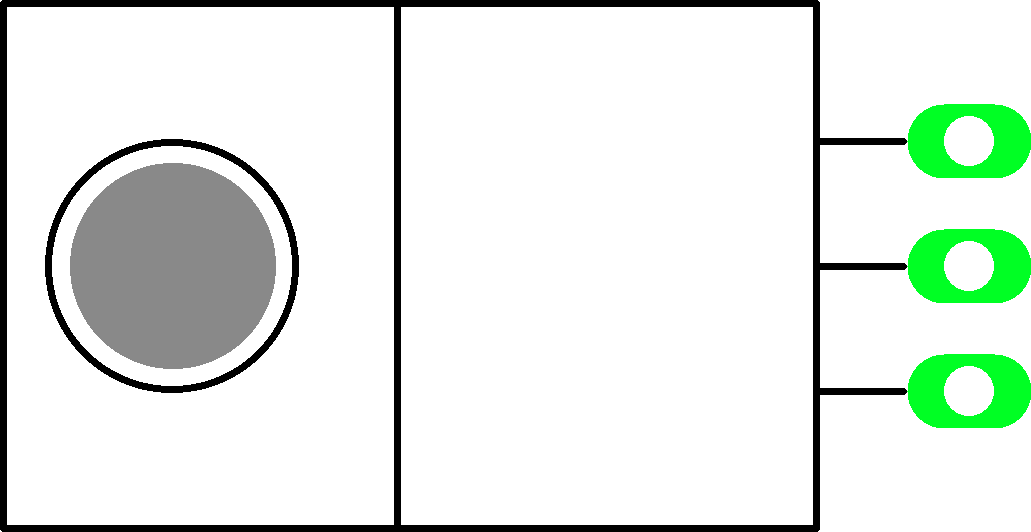
\includegraphics[height=1.2cm]{images/TO220_footprint_normal.png}
        }; &
        \node (pkg1) [anchor=center] {
         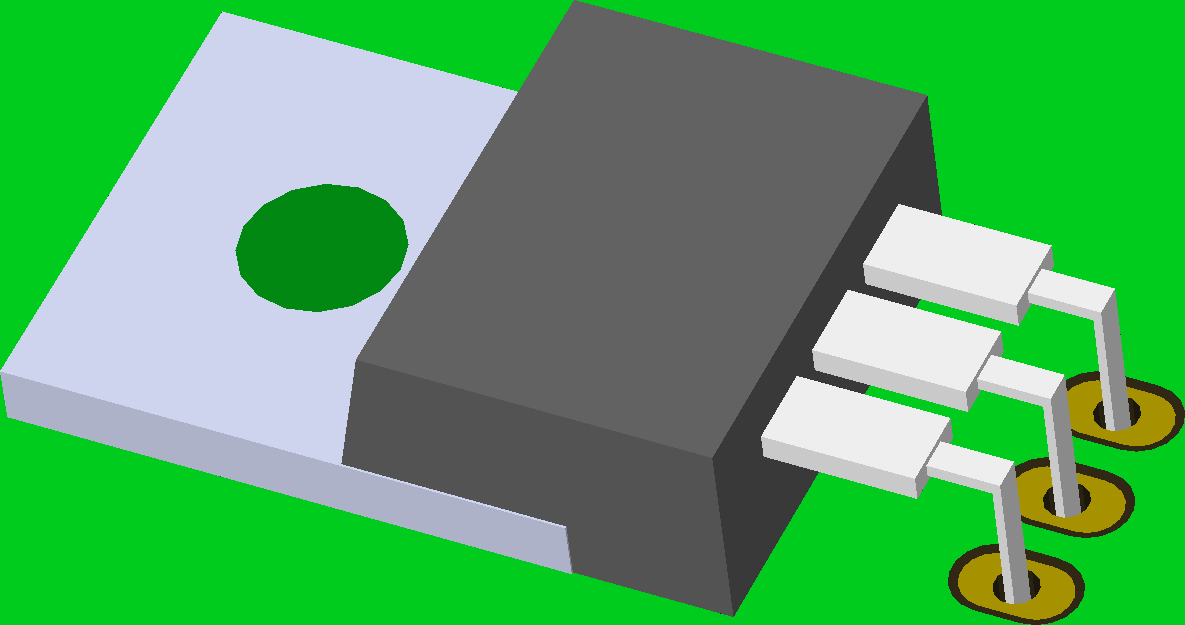
\includegraphics[height=1.2cm]{images/TO220_package_normal.png}
        }; \\

        \onslide<2->{\node (dev2) [lpbox, text width=2cm, anchor=center] {
          \textbf{IRLB8748} \\ (Mosfet)
        };} & &
        \onslide<3->{\node (fpt2) [anchor=center] {
          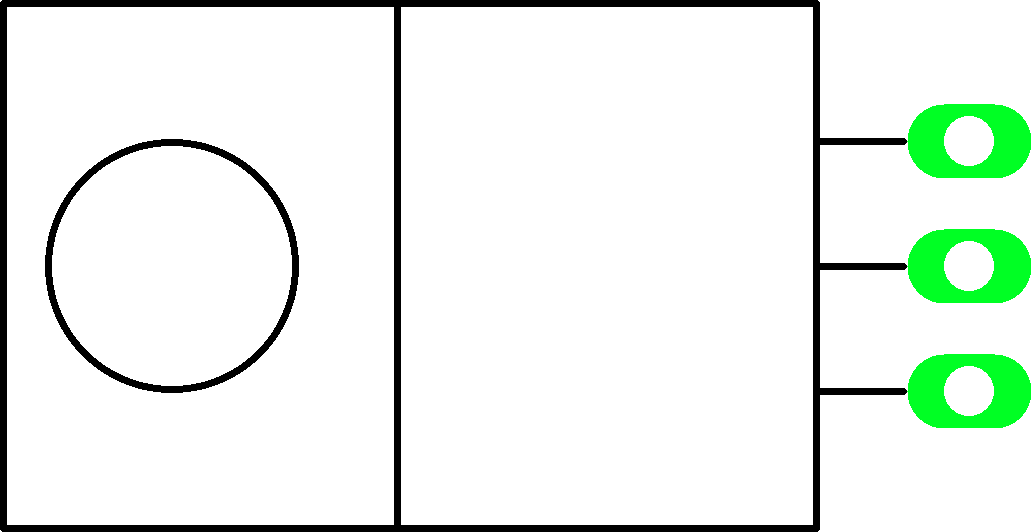
\includegraphics[height=1.2cm]{images/TO220_footprint_nohole.png}
        };} & \\

        \onslide<5->{\node (dev3) [lpbox, text width=2cm, anchor=center] {
          \textbf{MBR40250} \\ (Diode)
        };} & &
        \onslide<7->{\node (fpt3) [anchor=center] {
          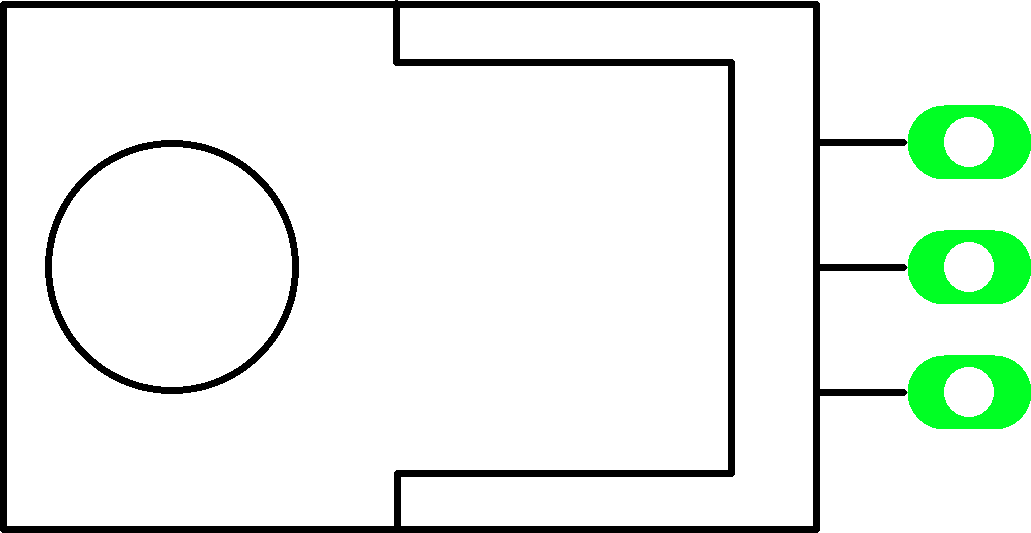
\includegraphics[height=1.2cm]{images/TO220_footprint_reverse.png}
        };} &
        \onslide<7->{\node (pkg3) [anchor=center] {
          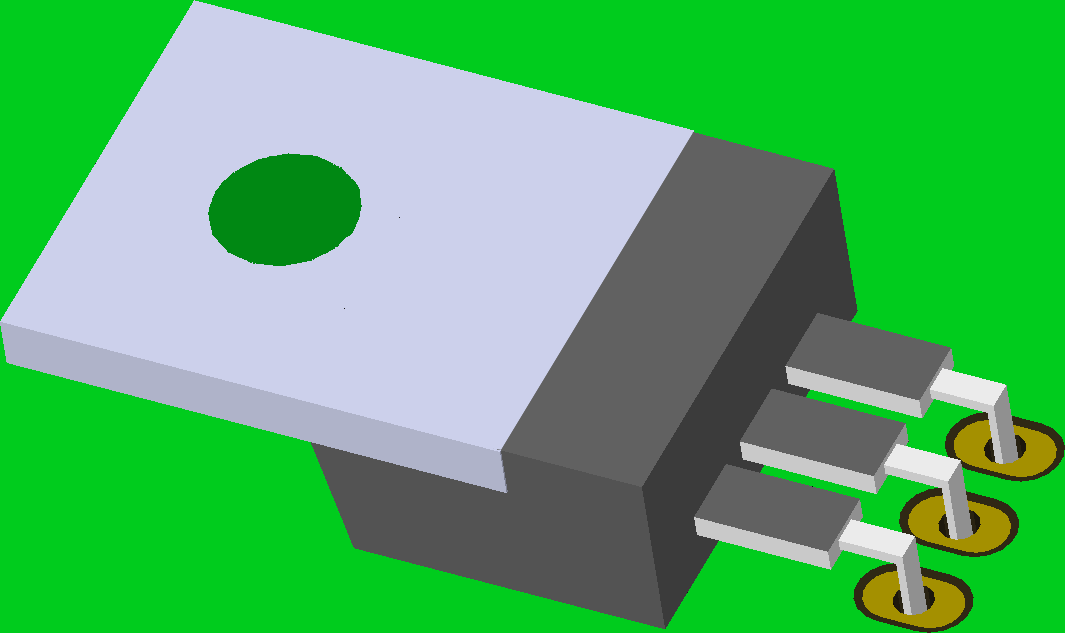
\includegraphics[height=1.2cm]{images/TO220_package_reverse.png}
        };} \\

        \onslide<6->{\node (dev4) [lpbox, text width=2cm, anchor=center] {
          \textbf{DS1821} \\ (Tsensor)
        };} & &
        \onslide<8->{\node (fpt4) [anchor=center] {
          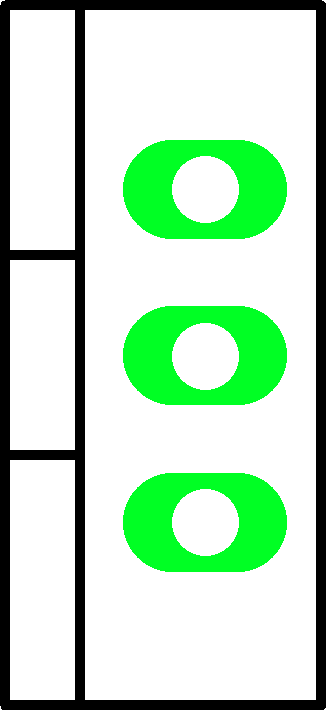
\includegraphics[height=1.2cm]{images/TO220_footprint_vertical.png}
        };} &
        \onslide<8->{\node (pkg4) [anchor=center] {
          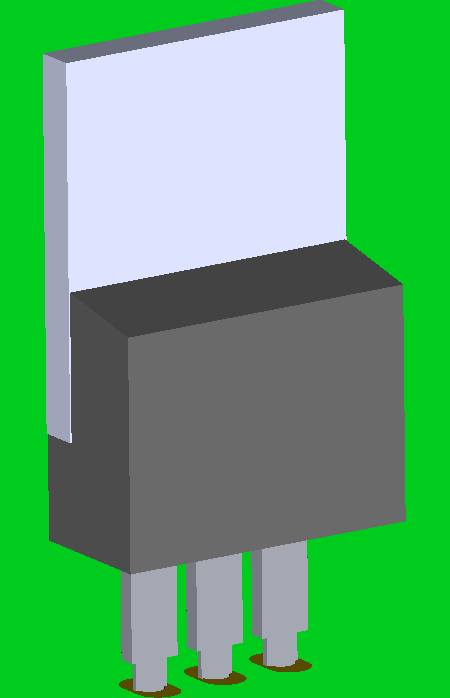
\includegraphics[height=1.2cm]{images/TO220_package_vertical.png}
        };} \\
      };

      \node (tdev) [above=12mm of dev1.center, anchor=center] {\textbf{Device}};
      \node (tfpt) [above=12mm of fpt1.center, anchor=center] {\textbf{Footprint}};
      \node (tmod) [above=12mm of pkg1.center, anchor=center] {\textbf{3D Model}};

      % package
      \onslide<9->{
        \node (tpkg) [anchor=center] at ($(tdev)!0.5!(tfpt)$) {
          \textbf{Package}
        };
        \node (pkg) [lpbox, anchor=center, rectangle split, rectangle split parts=4]
        at ($(dev2)!0.5!(fpt3)$) {
          \textbf{TO-220-3}
          \nodepart{two}   Pad \textbf{1}
          \nodepart{three} Pad \textbf{2}
          \nodepart{four}  Pad \textbf{3}
        };
      }
      \begin{pgfonlayer}{background}
        \coordinate (pkgbot) at ($(dev4.south)!0.5!(fpt4.south)$);
        \onslide<9->{
          \node[fill=yellow!60, fit=(tpkg)(pkg)(pkgbot), inner xsep=5mm, rounded corners] {};
        }
      \end{pgfonlayer}

      \begin{pgfonlayer}{background}
        % footprint -> 3d model
        \draw<1->[lpline, draw=red, ultra thick] (fpt1.east) -- (pkg1.west);
        \draw<3->[lpline, draw=red, ultra thick] (fpt2.east) -- (pkg1.west);
        \draw<7->[lpline, draw=red, ultra thick] (fpt3.east) -- (pkg3.west);
        \draw<8->[lpline, draw=red, ultra thick] (fpt4.east) -- (pkg4.west);

        % device -> footprint
        \draw<1-8>[lpline, draw=red, ultra thick] (dev1.east) -- (fpt1.west);
        \draw<2-8>[lpline, draw=red, ultra thick] (dev2.east) -- (fpt1.west);
        \draw<5-8>[lpline, draw=red, ultra thick] (dev3.east) -- (fpt1.west);
        \draw<6-8>[lpline, draw=red, ultra thick] (dev4.east) -- (fpt1.west);
        \draw<4-8>[lpline, draw=red, ultra thick] (dev1.east) -- (fpt2.west);
        \draw<4-8>[lpline, draw=red, ultra thick] (dev2.east) -- (fpt2.west);
        \draw<5-8>[lpline, draw=red, ultra thick] (dev3.east) -- (fpt2.west);
        \draw<6-8>[lpline, draw=red, ultra thick] (dev4.east) -- (fpt2.west);
        \draw<7-8>[lpline, draw=red, ultra thick] (dev1.east) -- (fpt3.west);
        \draw<7-8>[lpline, draw=red, ultra thick] (dev2.east) -- (fpt3.west);
        \draw<7-8>[lpline, draw=red, ultra thick] (dev3.east) -- (fpt3.west);
        \draw<7-8>[lpline, draw=red, ultra thick] (dev4.east) -- (fpt3.west);
        \draw<8-8>[lpline, draw=red, ultra thick] (dev1.east) -- (fpt4.west);
        \draw<8-8>[lpline, draw=red, ultra thick] (dev2.east) -- (fpt4.west);
        \draw<8-8>[lpline, draw=red, ultra thick] (dev3.east) -- (fpt4.west);
        \draw<8-8>[lpline, draw=red, ultra thick] (dev4.east) -- (fpt4.west);

        % device -> package
        \draw<9->[lpline, draw=red, ultra thick] (dev1.east) -- (pkg.west);
        \draw<9->[lpline, draw=red, ultra thick] (dev2.east) -- (pkg.west);
        \draw<9->[lpline, draw=red, ultra thick] (dev3.east) -- (pkg.west);
        \draw<9->[lpline, draw=red, ultra thick] (dev4.east) -- (pkg.west);

        % package -> footprint
        \draw<9->[lpline, draw=red, ultra thick] (pkg.east) -- (fpt1.west);
        \draw<9->[lpline, draw=red, ultra thick] (pkg.east) -- (fpt2.west);
        \draw<9->[lpline, draw=red, ultra thick] (pkg.east) -- (fpt3.west);
        \draw<9->[lpline, draw=red, ultra thick] (pkg.east) -- (fpt4.west);
      \end{pgfonlayer}
    \end{tikzpicture}
  \end{center}
\end{frame}
